\scanpage{7}
\mspage{1}

% This entirely handwritten page has no handwriting envelope (briefv06).
% Main 01: certain accent, unresolved direction; two quotation ticks each side.
Let \(M\) be a category (``\unsure{models|models}''). We assume

% Main 02: accent direction remains uncertain; no point after monomorphique.
(i) Every \unsure{arrow|arrow} of \(M\) is monomorphic

% Main 03: abbreviated old word, uncertain old stop, raised end without stop.
(ii) Every \deleted{\unsure{automorphism|automorphism}}\inserted{endomorphism} of an element of \(M\) is the identity.

% Main 04: the reduced internal strokes do not resolve par.
Example : \(M\) a category defined \unsure{by} an ordered set

% Main 05: quotation ticks and a real blank, without a hyphen, in sous objets.
% Main 06: no point follows the terminal tilded D of the identification.
For every \(D\in\mathrm{Ob}\,M\), let \(\widetilde D\) be the set (ordered by ``inclusion'') of subobjects of \(D\). We identify \(D\) with the greatest element of \(\widetilde D\)

Let \(D',D\in\mathrm{Ob}\,M\), then the map
% Main 07: a literal two-row map; M belongs under the final m of Hom.
% Lower u is indented; its barred shaft starts farther left and runs longer.
% The star is far left between row levels; the upper target has no comma.
\diagram{\begin{tikzcd}[ampersand replacement=\&,row sep=0pt,column sep=0pt]
{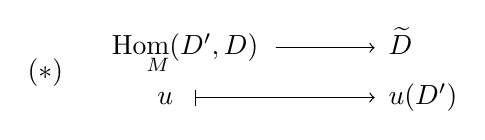
\begin{tikzpicture}[x=1em,y=1em,line width=.45pt,
 line cap=round,line join=round]
\node[anchor=base west,inner sep=0pt,outer sep=0pt] (homHo)
 at (0,0) {$\mathrm{Ho}$};
\node[anchor=base west,inner sep=0pt,outer sep=0pt] (homLast)
 at (homHo.base east) {$\mathrm m$};
\node[anchor=base west,inner sep=0pt,outer sep=0pt] (homArgs)
 at (homLast.base east) {$(D',D)$};
\node[anchor=north,inner sep=0pt,outer sep=0pt]
 at ([yshift=-.12em]homLast.south) {$\scriptstyle M$};
\node[anchor=base west,inner sep=0pt,outer sep=0pt]
 at (10,0) {$\widetilde D$};
\draw[->] ([xshift=.65em,yshift=.25em]homArgs.base east)--(9.5,.25);
\node[anchor=base west,inner sep=0pt,outer sep=0pt]
 at (1.65,-1.8) {$u$};
\draw[|->] (3,-1.55)--(9.5,-1.55);
\node[anchor=base west,inner sep=0pt,outer sep=0pt]
 at (10,-1.8) {$u(D')$};
\node[inner sep=0pt,outer sep=0pt] at (-2.4,-.65) {$(\ast)$};
\end{tikzpicture}}
\end{tikzcd}}
% Main 08: mixed first enclosure retained ahead of the two matched alternatives.
% Main 09: ens has no stop; the canceled de remains low-confidence;
% Phi is resolved, and inserted M- attaches before isomorphes.
is injective by \unsure{(i]|[i]|(i)}(ii), its image consists of the set \deleted{\unsure{of}}
\(\Phi_{D'}(D)\subset\widetilde D\)
of subobjects \(\Delta\) of \(D\) which are \inserted{\(M\)-}isomorphic to \(D'\).

\deleted{Let \(K\) be an ordered set}

% Main 10--13 and 26: plain live N, deleted I, interlinear preordonne;
% the inserted sentence has only ordonne underlined; preceding M has its point.
Let \(N\)\deleted{\(I\)} be the \inserted{preordered} set of isomorphism classes of objects of \(M\). \inserted{It is in fact \uline{ordered}, thanks to (ii).}
% Main 14--18: unresolved forall/H, doubled N, canceled e/s, old D and live M;
% a raised star over n, and the first isom without a stop.
For \(\unsure{\forall|\mathrm H}\ n\in\mathbb N\), an\deleted{\unsure{e|s}} object \(D_n\) of \deleted{\(D\)}\(M\) of class \(\overset{\ast}{n}\) is determined up to unique isomorphism,
% Main 19: reduced a/colon cluster plus a separate low down-right stroke.
% The literal stroke is neither a character candidate nor a therefore sign.
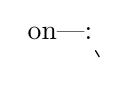
\begin{tikzpicture}[baseline=(causecluster.base),x=1em,y=1em,
 line width=.45pt,line cap=round]
\node[anchor=base west,inner sep=0pt,outer sep=0pt] (causecluster)
 at (0,0) {\unsure{on|:}};
\draw ([xshift=.12em,yshift=-.4em]causecluster.south east)
 --([xshift=.25em,yshift=-.62em]causecluster.south east);
\end{tikzpicture} account of (ii),
% Main 20--22: ens without a stop; plain tilde D_n equals doubled J_n;
% resolved defini and the second isom without a stop.
thus the ordered set \(\widetilde D_n=\mathbb J_n\) is defined up to unique isomorphism.
% Main 23: dotted plui remains the first candidate; comma and old une are deleted.
We therefore have \deleted{\unsure{more|plui}, a}\inserted{a} family
% Main 24: the family is a separate display.
\[
(\mathbb J_n)_{n\in\mathbb N}
\]
% Main 25: retain the observed footer wording and punctuation.
of ordered sets, indexed by the ordered set \(\mathbb N\).
% archive sheet number: 6
